\documentclass{beamer}
\usepackage{beamerthemesplit}
\usepackage{booktabs}
\usepackage{graphicx}
\usepackage{transparent}
\usepackage{bbold}
\usepackage[italian]{babel}
\usepackage[utf8x]{inputenc}
\usepackage{listings}
\usepackage{tikz}
\usetikzlibrary{fit, shapes, arrows, patterns, matrix}
\usepackage{amsmath,amsfonts,amssymb}
\usepackage{pgfplots}
\usepackage{scalefnt}
\usepackage{color}
\usepackage{xcolor}
\usepackage{multicol}
\usepackage{bm}
\usepackage{changepage}

\title[Algoritmi]{Algoritmi di feature selection}
\institute{
\begin{small}
Corso di Laurea in Informatica Magistrale
\end{small}}
\author{\textbf{Simone Rutigliano}}
\date{\tiny{\today}}

\usebackgroundtemplate{
%    \transparent{0.12}{
     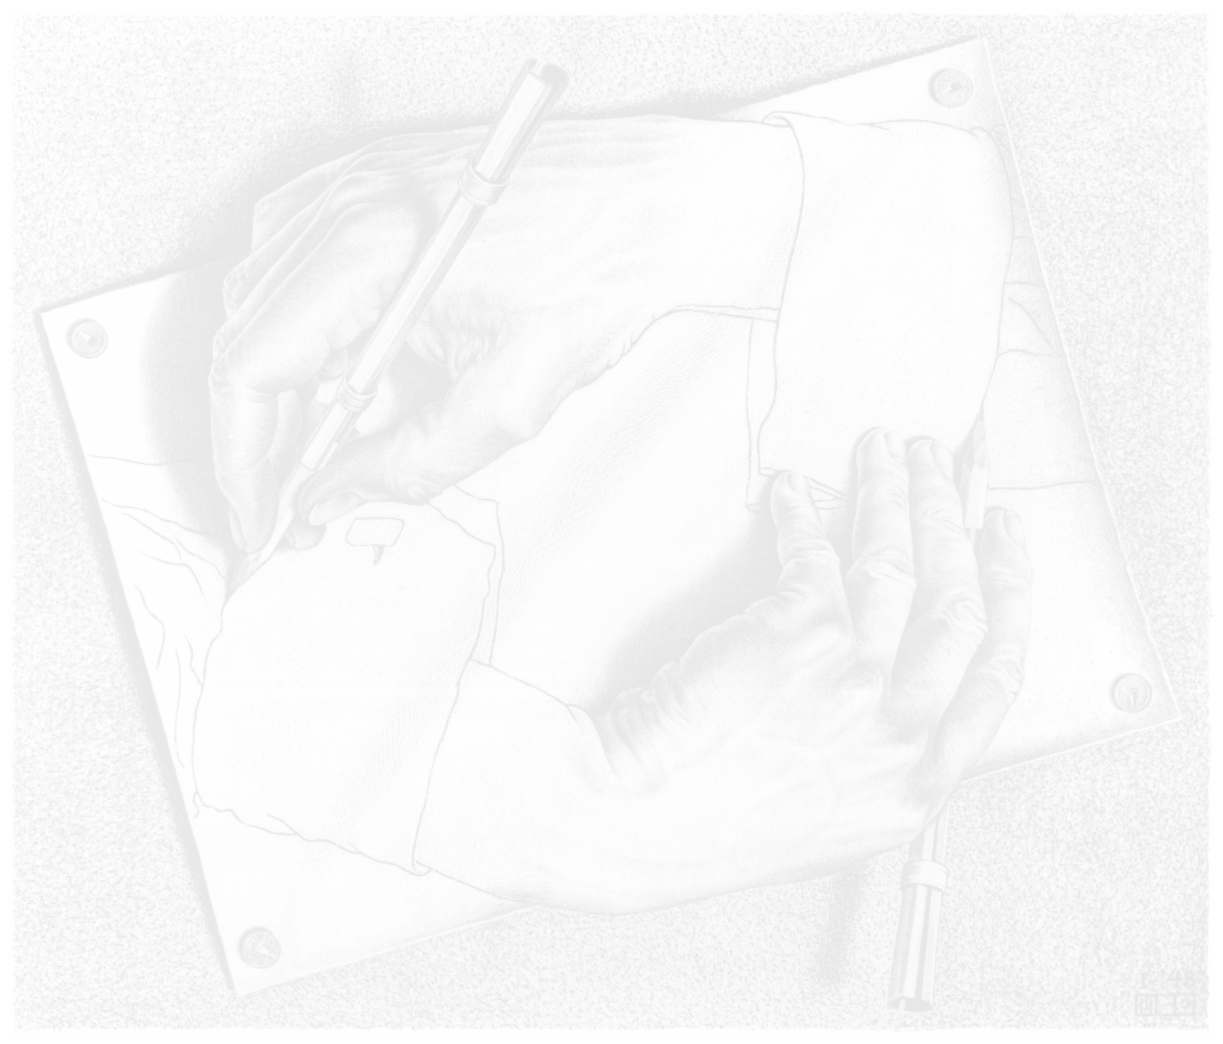
\includegraphics[width=\paperwidth, height=\paperheight]{./figure/theme/escher_hands_tr.png}
%    }
}

%\usetheme{Hannover}
\usetheme{Copenhagen}
\usecolortheme{seahorse}
\usecolortheme{rose}
%\usetheme{Frankfurt}
%\usecolortheme{beetle}

%\useoutertheme[subsection=false]{smoothbars}
%\useoutertheme[subsection=false]{smoothtree}
\useoutertheme{shadow}
\setbeamercovered{dynamic}

\pgfdeclareimage[height=1cm]{logo}{figure/theme/logo}
\logo{\pgfuseimage{logo}}

\begin{document}

%%%%%%%%%%%%%%%%%%%%%%%%%%%%%%%%%%%%%%%%%%%%%%%%%%%%%

\begin{frame}
\maketitle
\end{frame}

%%%%%%%%%%%%%%%%%%%%%%%%%%%%%%%%%%%%%%%%%%%%%%%%%%%%%

\begin{frame}
\frametitle{Outline}
	\begin{columns}
		\begin{column}{0.4\textwidth}
			\begin{equation*}
			\qquad \textbf{Java}
			\begin{cases} 
			PageRank
			\\ 
			HITS
			\\
			SALSA
			\\
			ReConRank
			\\
			SimRank
			\\
			TripleRank
			\\
			mRMR
			\\
			PICSS
			\end{cases}
			\end{equation*}
		\end{column}
		\begin{column}{0.8\textwidth}
			\begin{equation*}
			\qquad \textbf{RapidMiner}
			\begin{cases} 
			SHSEL \begin{cases} 
			Information ~Gain \\ \mbox{\emph{Correlation}}
			\end{cases}
			\\~\\
			Greedy Top Down
			\end{cases}
			\end{equation*}
		\end{column}
	\end{columns}
\end{frame}

\section{Algoritmi Java}
\subsection{PageRank}
\begin{frame}
	\frametitle{PageRank}
	Implementazione del \emph{Wrapper Model}: 
	\begin{itemize}
		\item Utilizzare lo stesso algoritmo sia per la feature selection sia per la fase di raccomandazione
		\item Subset ottimizzato per la raccomandazione
	\end{itemize}
\end{frame}
\subsection{HITS}
\begin{frame}
	\frametitle{HITS}
	Creazione del subset attraverso l'utilizzo dell'algoritmo di \emph{Hyperlink-Induced Topic Search} basato sul \emph{ranking} di risorse in base a due metriche:
	\begin{itemize}
		\item Hub
		\item Authority
	\end{itemize}
	Implementazioni trovate:
	\begin{itemize}
		\item \url{http://goo.gl/4pWAq4}
		\item \url{http://goo.gl/qSDXru}
	\end{itemize} 
\end{frame}
\subsection{SALSA}
\begin{frame}
	\frametitle{SALSA}
	\begin{itemize}
		\item Combinazione di HITS e PageRank
		\item Usa i punteggi di Hub e Autority
		\item Crea un grafo bipartito $G=(V_1 \cup V_2,E)$ dove \begin{itemize}
			\item $V_1$ rappresenta il set degli Hub
			\item $V_2$ rappresenta il set degli Autority
			\item Una risorsa può essere contenuta sia in un set che nell'altro
		\end{itemize}
	\end{itemize}
	Implementazione trovata:
	\begin{itemize}
	\item \url{http://goo.gl/DtHa4K}
	\end{itemize}
\end{frame}
\subsection{ReConRank}
\begin{frame}
	\frametitle{ReConRank}
	Tratto dal paper \cite{Hogan06reconrank:a}
	\begin{itemize}
	\item 	Basato su due ranking:
	\begin{itemize}
		\item \textbf{ResourceRank} : Associa uno score basato sul PageRank alle risorse del grafo RDF
		\item \textbf{ContextRank} : Permette di inglobare la provenienza del contenuto semantico nel calcolo del ranking
	\end{itemize}
	\item Computazione molto onerosa
	\item Implementazioni trovate
	\begin{itemize}
		\item \url{http://goo.gl/PnZfNc}
		\item \url{http://goo.gl/oCwQWe}
	\end{itemize}
\end{itemize}
\end{frame}

\subsection{SimRank}
\begin{frame}
	\frametitle{SimRank}
	Tratto dal paper \cite{Jeh:2002:SMS:775047.775126}
	Algoritmo per il calcolo di similarità tra due nodi all'interno di un grafo $G$
	\begin{itemize}
		\item Esegue un random walk con ripartenza da un nodo fissato $u$ su un grafo k-partito
		\item Gli score risultati misureranno la similarità tra il nodo $u$ e tutti gli altri nodi del grafo
	\end{itemize}
	Implementazione trovata:
	\begin{itemize}
		\item \url{http://goo.gl/9cLDda}
	\end{itemize}
\end{frame}
\subsection{TripleRank}
\begin{frame}
	\frametitle{TripleRank}
	Tratto dal paper \cite{Franz:2009:TRS:1693684.1693699}
	\begin{itemize}
		\item Consiste in una generalizzazione di HITS nel contesto dei Linked Data
		\item The algorithm was evaluated for faceted browsing and filtering semantic relations for a better Linked Data exploration experience
	\end{itemize}
	Implementazione trovata:
	\begin{itemize}
		\item \url{http://goo.gl/Pb3vEr} (Richiede l'utilizzo di Matlab)
	\end{itemize}
\end{frame}
\subsection{mRMR}
\begin{frame}
	\frametitle{mRMR}
	Tratto dall'articolo \cite{Peng05featureselection} e approfondito in \cite{SRutigliano2014}
	\begin{itemize}
		\item Consiste nel calcolo della
		\begin{itemize}
			\item \textbf{minima ridondanza} tra le features
			\item \textbf{massima rilevanza} delle features con la classe target
		\end{itemize}
		Implementazione trovata:
		\begin{itemize}
			\item \url{http://goo.gl/YQUx1s}
		\end{itemize}
\end{frame}


\subsection{PICSS}
\begin{frame}
	\frametitle{PICSS}
	Ranker by Information Content (PICSS We propose our partitioned information 
	content (PIC)-based semantic similarity measure, called PICSS , which is a 
	combination of feature- and information content-based approaches. Feature in
	comune per la similarità
	
	 Pesa gli archi con information content e similarità tra feature
\end{frame}
\section{RapidMiner - LOD Extension}
\subsection{SHSEL - IG}
\begin{frame}
	\frametitle{SHSEL - Information Gain}
	University of Mannheim
\end{frame}
\subsection{TSEL - IG}
\begin{frame}
	\frametitle{TSEL - Information Gain}
	University of Mannheim
\end{frame}
\subsection{Greedy Top Down}
\begin{frame}
	\frametitle{Greedy Top Down}
	University of Mannheim
\end{frame}
%%%%%%%%%%%%%%%%%%%%%%%%%%%%%%%%%%%%%%%%%%%%%%%%%%%%%
\begin{frame}{Bibliography}
	\frametitle{References}
	\bibliographystyle{alpha}
	\bibliography{mybib}
\end{frame}
\end{document}
